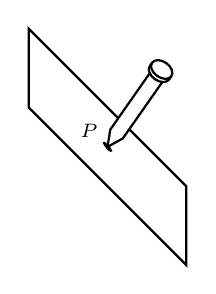
\begin{tikzpicture}
	
	\begin{scope}[cm={-1,1,0,1,(0,0)},yscale=.5]
		\draw [thick](-1,-1) rectangle (1,1);
		\filldraw [black] (0,0) circle (1.5pt) node [above left] {\scriptsize $P$};
	\end{scope}
	\begin{scope}[rotate=-35]
	\begin{scope}[xscale=.15,yscale=.1,shift={(0,12)}]
	\filldraw [draw=black,fill=white,thick] (-.65,0) -- (-.65,-10)--(0,-12)--(.65,-10)--(.65,0);
	\filldraw[draw=black,thick,fill=white] (1,0) arc (0:180:1) -- ++(0,-.5) arc (180:360:1) --cycle;
	\draw [thick] (1,0) arc (0:-180:1);
	\end{scope}
	\end{scope}
\end{tikzpicture}
